\documentclass{article}

\usepackage{graphicx}
\usepackage{algorithm}
\usepackage{algpseudocode}
\usepackage{authblk}
\usepackage{url}
\usepackage[utf8]{inputenc}
\usepackage{color}
\usepackage{amsmath}

\title{AI Assignment-3 Report}
\vspace{20pt}
\vspace{20pt}
\date{\today}
\author{Team -14 \\Tabish Khalid Halim , \\ 200020049 \\ Anand Hegde , \\ 200020007}
\vspace{20pt}
\affil{Department of Computer Science, IIT Dharwad}
\begin{document}

\maketitle
\pagenumbering{gobble}
\newpage
\tableofcontents

\newpage
\pagenumbering{arabic}
\section{Problem Statement}
We are given the question to find the satisfiability of a Uniform 4-SAT \{which is a family of SAT problems distribution obtained from generating 4-CNF formulae randomly.\}
\\So , if all the clauses are true , then we can prove the satisfability of a formula.
\vspace{10pt}
\section{Approach}
The basic approach we used for the A.I assignment is to use the concept \\of Exploration and 
apply VND \{Variable Neighborhood Descent\}, Beam Search and Tabu Search.
\vspace{10pt}
\subsection*{State Space}
A state space is the set of all configurations that a given problem and its \\environment could achieve .
\vspace{10pt}
\\We have been given with the fact that there are n bits of strings of 0s and 1s for an n variable state space.
\\Thus , the total number of state spaces in the state space set is $2^n$ .
\subsection*{Start \& Goal node}
The Start node is a randomly generated n bit string which will be
a part of the state space that will be 
given in 'input.txt' file.
\\The Goal Node is a part of the state space that represents the final/goal state to be reached through
our algorithm .
\\One such example is the following :
\\For $n=5$ i.e. 5 variables,
\\Start Node :
\\10001
\\Goal Node :
\\10101
\newpage
\section{Pseudo Code}
The main pseudo code used in our assignment is as follows :
\subsection*{move\_gen function}
\vspace{5pt}
def move\_gen(state,bits\_toggled):
\vspace{5pt}
    \vspace{2pt}
    \\ \hspace*{20pt}neighbors = [ ]
    \vspace{2pt}
    \\ \hspace*{20pt}comb = iter.combinations(0 to total no. of states)),bits\_toggled)
    \vspace{2pt}
    \\ \hspace*{20pt}for i in comb:
    \vspace{2pt}
    \\ \hspace*{30pt}new= state
    \vspace{2pt}
    \\ \hspace*{30pt}for j in i:
    \vspace{2pt}
    \\ \hspace*{40pt}j= int(j)
    \vspace{2pt}
    \\ \hspace*{40pt}new= new[:j]+str((int(new[j])+1)\%2)+new[j+1:]
    \vspace{2pt}
    \\ \hspace*{70pt}neighbors.append(new)
    \vspace{2pt}
    \\ \hspace*{20pt}return neighbors

\subsection*{goal\_state function}
    \vspace{5pt}
    def goal\_state(formula,inpu):
        \vspace{5pt}
        \\ \hspace*{20pt}global no\_clauses
        \vspace{5pt}
        \\ \hspace*{20pt}if(no\_of\_clauses(formula,inpu)==no\_clauses):
        \vspace{5pt}
        \\ \hspace*{30pt} return 1
        \vspace{5pt}
        \\ \hspace*{20pt} return 0
\newpage
\section{Heuristic function}
\vspace{10pt}
We are considering the no. of satisfied clauses as the heuristic for our program.
If the heuristic value is n , i.e. no. of clauses, then that node is our goal state.
\subsection*{Pseudo Code:}
\vspace{5pt}
    def evaluate\_clause(clause,inpu):
        \vspace{2pt}
        \\ \hspace*{20pt}for i in clause:
        \vspace{2pt}
        \\ \hspace*{30pt}if(i$>$0):
        \vspace{2pt}
        \\ \hspace*{50pt} if(inpu[i-1]=='1'):
        \vspace{2pt}
        \\ \hspace*{70pt} return 1
        \vspace{2pt}
        \\ \hspace*{30pt} else:
        \vspace{2pt}
        \\ \hspace*{50pt} if(inpu[i-1]=='1'):
        \vspace{2pt}
        \\ \hspace*{70pt} return 1
        \vspace{2pt}
        \\ \hspace*{20pt} return 0
\vspace{15pt}
        \\def no\_of\_clauses(all\_clauses,inpu):
            \vspace{2pt}
            \\ \hspace*{20pt}no = 0
            \vspace{2pt}
            \\ \hspace*{20pt}for i in clause:
            \vspace{2pt}
            \\ \hspace*{30pt}if(evaluate\_clause(i,inpu)):
            \vspace{2pt}
            \\ \hspace*{50pt} no += 1
            \vspace{2pt}
            \\ \hspace*{20pt} return no
\newpage
%\section{VND\hspace*{5pt} \{Variable Neighborhood Descent\}}
%We already know that in order to escape the local maxima 
%we have to make the neighborhood denser which can be achieved 
%by increasing the no. of bits to be toggled .
\section{Beam Search Analysis}
The time taken to reach the goal state increases exponentially as the input size increases.
As the width of the beam search is increased, the probability of getting the best node also increases because the more the
nodes get explored, more is the chance of finding the goal state.
\\Also , as the width of the beam search is increased , we see that the computation time and space complexity of the beam search to reach the goal state also increases.
\\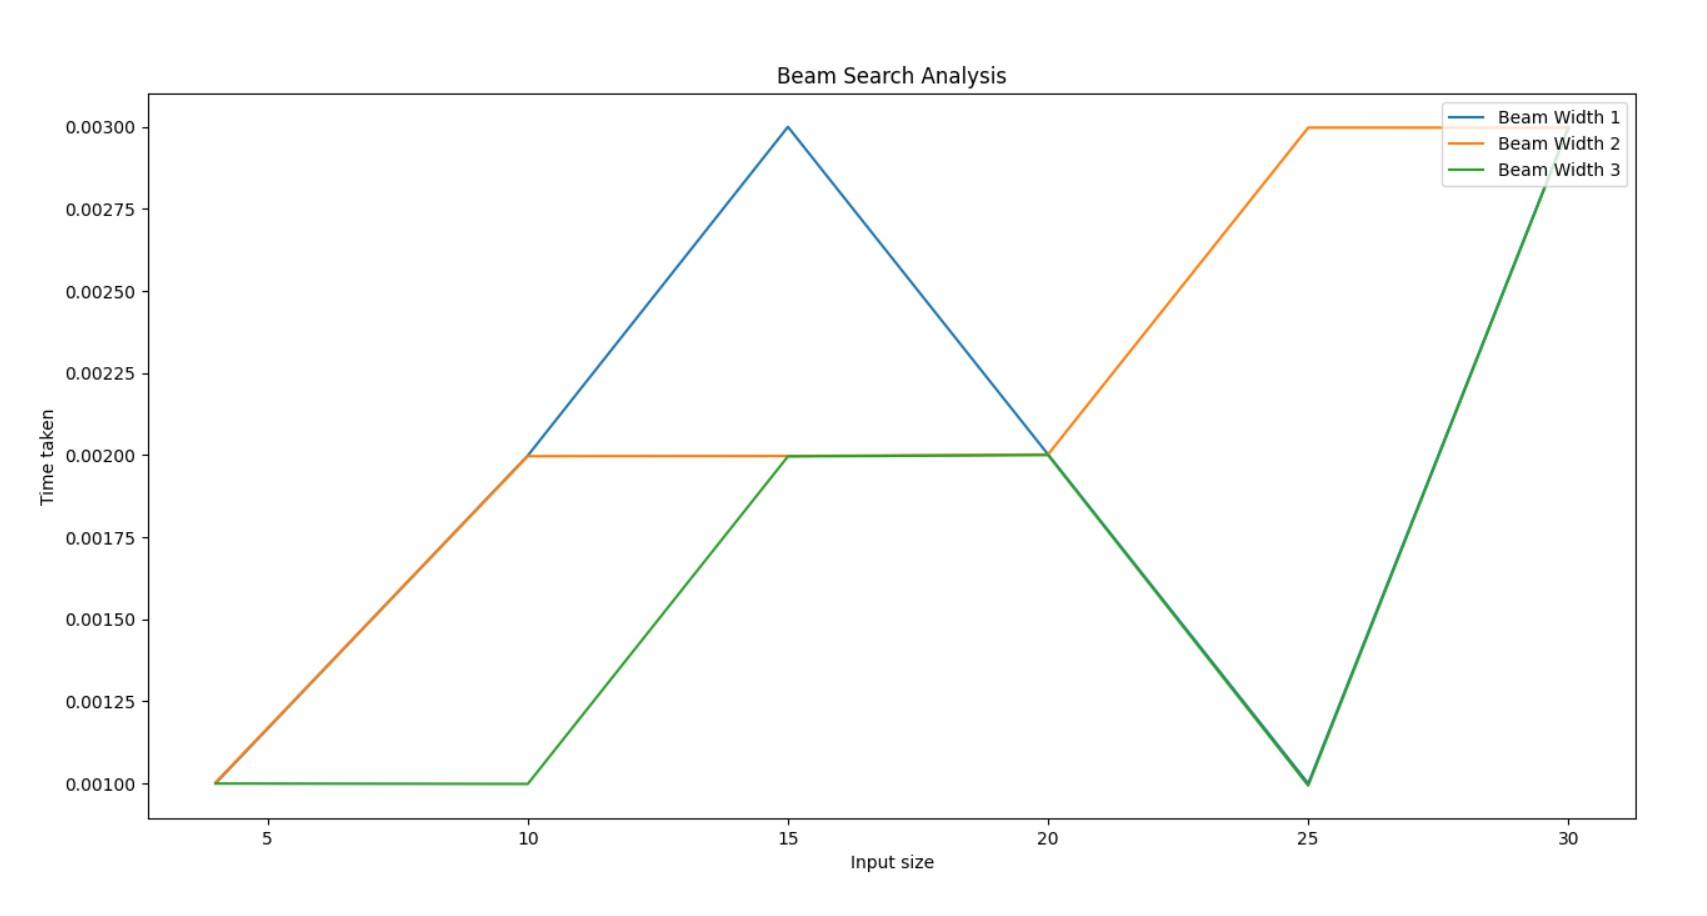
\includegraphics[scale=0.3]{BeamSearch.jpg}
\newpage
\section{Tabu Search Analysis}
We have compiled the following results for Tabu Search with different values of Tabu Tenure .
\vspace*{10pt}
\\\hspace*{50pt}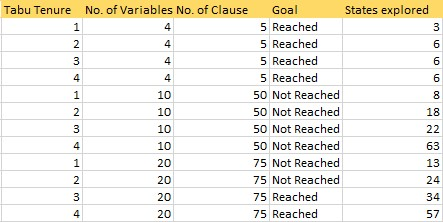
\includegraphics{Table2.jpg}
\vspace*{10pt}
\\Here is a graph for different Tabu Tenures with number of clauses = 10. 
\\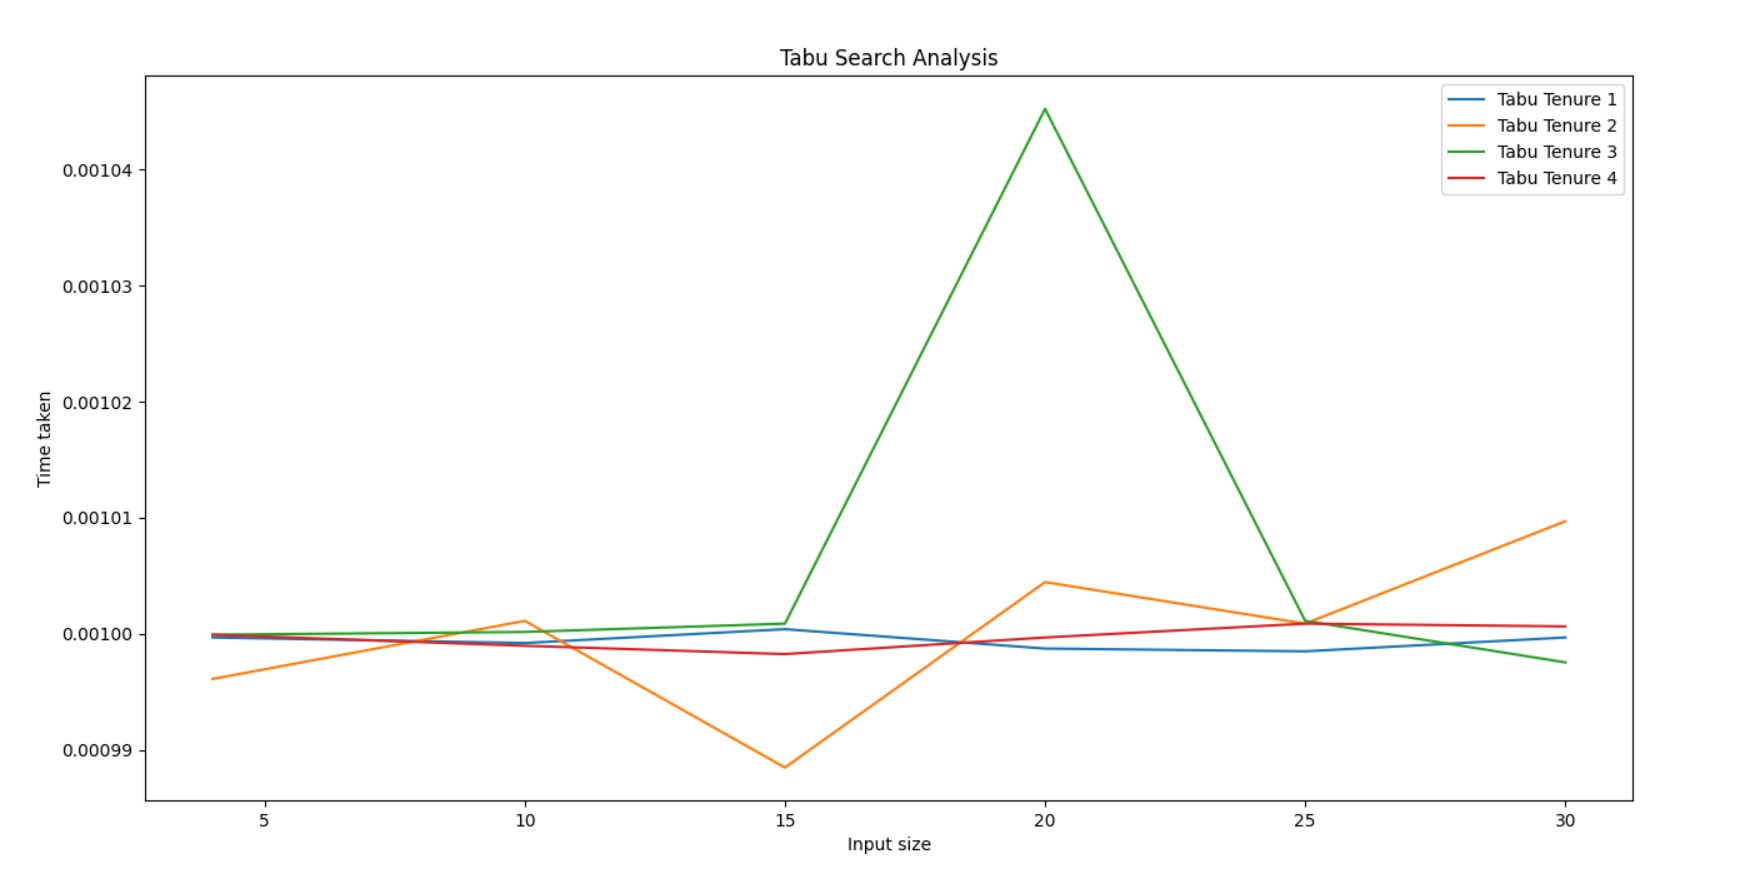
\includegraphics[scale=0.35]{TabuSearch.jpg}
\newpage
\section{Analysis \& Observations}
\vspace{5pt}
Based on observation , we have compiled the following data pertaining to VND, Beam Search and Tabu Search :
\vspace*{10pt}
\\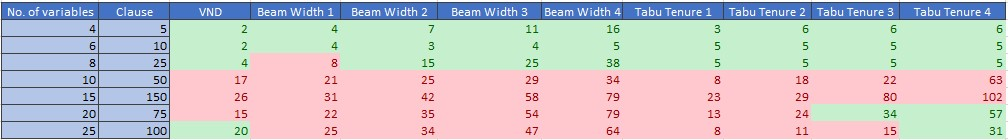
\includegraphics[scale=0.7]{Table1.jpg}
\vspace*{10pt}
\\In the above table , the green cells represents success of finding the goal state and the red cells represents the failure of reaching to the goal state.
\vspace*{10pt}
\\Here is the graphical analysis for VND. 
\\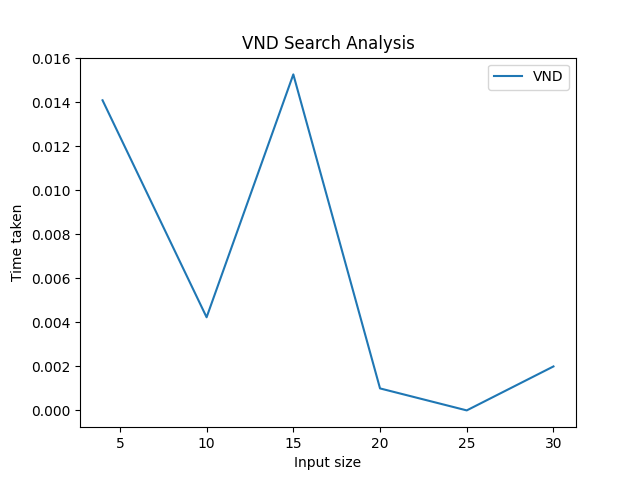
\includegraphics{VND.png}
%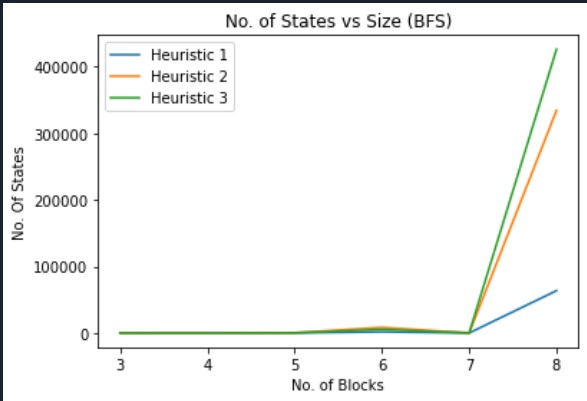
\includegraphics{Graph1.jpg}
\newpage
\section{Results}
\vspace{20pt}
The following conclusions have been made after evaluation of our program :
\begin{description}
    \item[VND \{Variable Neighborhood Descent\} :] If there exist a solution to reach the goal state then this algorithm is considerably fast 
    but , if there does not exist a solution then, it will be very slow.  
    \item[Beam Search Algorithm :] As the beam width of Beam Search Algorithm increases , the time taken also increases but the possibility to reach the goal state will also increase.
    \item[Tabu Search Algorithm :] If the tabu tenure is very low , then the algorithm will roam around the local optima but if the tabu tenure very high then the algorithm will explore very few nodes
    but for a well chosen tenure , we will reach the goal state in a very short amount of time. 
    \\We can conclude that the optimal value of the Tabu Tenure should be around :
    No. of literals/5 \{ if $n\geq10$ , otherwise 2\}
\end{description}
%\vspace{20pt}
\section{Conclusion}
All the above described algorithms help to overcome the problem of escaping local minima and
they work reasonably well when the hyper-parameters like Tabu Tenure and Beam Width are chosen wisely. 
\newpage
\section{References}
\vspace{30pt}
\begin{itemize}
    \item \url{http://geeksforgeeks.com}
    \item \url{https://wikipedia.org}
    \item \url{https://stackoverflow.com}
\end{itemize}
\end{document}